% ======================================================================================================
\section{Identifiability}\label{sec:ident}
% ======================================================================================================

\subsection{What one record can and cannot determine}

In the loop band the beam changes the recorded response by a few percent; the response is set by the loop. For a complex-linear loop the five parameters $G$, $\theta$, $\tau$, $\QL$ and $\Delta f$ are determined by one record: at \SI{22}{mA} the loop band of a single record returns them with statistical errors of \sdG{} in $G$, \ang{\sdTheta} in $\theta$, \SI{\sdTau}{ns} in $\tau$, \sdQL{} in $\QL$ and \SI{\sdDf}{kHz} in $\Delta f$. A compressed klystron and a one-dimensional excitation change this. For cavities on tune and no beam, $\mat M=m(s)\mat A$ with the scalar $m=Gc\,Z/R_L$ and the constant matrix $\mat A=\mat R(\theta)\mat K$. With $\mat A=\mat V\mathrm{diag}(\lambda_1,\lambda_2)\mat V^{-1}$, Eq.~\eqref{eq:recorded} becomes
\begin{equation}\label{eq:twomodes}
H(f)=-\sum_{i=1,2}w_i(\alpha)\,\frac{m(s)\lambda_i}{1+m(s)\lambda_i},
\end{equation}
a weighted sum of two closed-loop responses whose loop gains are the eigenvalues of $\mat A$. The four quantities $\theta$, $\gA$, $\kAP$, $\alpha$ (with $G$) are carried by two complex gains and their weights, and the shapes of the two terms differ only through their bandwidths $(1+\lambda_i)\omega_{1/2}$. A single complex-linear response with an effective gain and phase approximates such a sum closely, which is why a linear model with effective parameters fits each record (Sec.~\ref{sec:explain}). Detuning and beam break the symmetry only partially. Moreover, the phase-path gain of the klystron and the controller gain enter only as a product, and the synchrotron frequency enters the loop band only through the beam's small contribution there.

\subsection{What operating-condition diversity adds}

A change of the loop-phase setting rotates $\mat A$ by a known angle, and a change of the loop-gain setting scales it by a known factor; neither changes $\gA$, $\kAP$ or $\alpha$ at a given operating point. Each additional record at the same operating point therefore adds \nCellsRecord{} complex data points but only one parameter, $\theta$, and moves the two eigenvalues of Eq.~\eqref{eq:twomodes} in a prescribed way. Records at other beam currents share the station constants and constrain the detuning through the beam loading.

Figure~\ref{fig:ident} quantifies the effect for the compression of the klystron at \SI{497}{mA}. The profile likelihood of $\gA$ is computed with every other parameter re-optimized~\cite{Raue2009}. From the loop band of one record, $\gA$ is bounded only from below ($\gA>\gaOneWLo$ at 95\%), a linear klystron fits as well as a compressed one ($\Delta\chi^2=\gaOneWAt$ at $\gA=1$), $\kAP$ is unconstrained, and the normalized Fisher information has condition number $\condOneW$. Adding the near band of the same record narrows $\gA$ to \gaOneLo--\gaOneHi{} ($\Delta\chi^2=\gaOneAt$ at $\gA=1$). The seven records of the \SI{497}{mA} gain and phase scan give \gaScanLo--\gaScanHi{} ($\Delta\chi^2=\gaScanAt$), and all eighteen records \gaAllLo--\gaAllHi{} ($\Delta\chi^2=\gaAllAt$). The compression is therefore identified, and robustly so: its value moves by less than 0.04 between data sets. The AM/PM coefficient is not. It is bounded within each data set ($\kAP=\kapScanOpt$, 95\% interval \kapScanLo{} to \kapScanHi{}, from the scan; \kapAllOpt, \kapAllLo{} to \kapAllHi{}, from all records), but it moves between data sets together with the loop phase at \SI{497}{mA}, because a rotation of the loop and an amplitude-to-phase conversion in the klystron produce similar changes of the projected response. The closed-loop records therefore identify the compression but not the AM/PM conversion, which has to come from elsewhere.

\begin{figure}[tb]
\centering
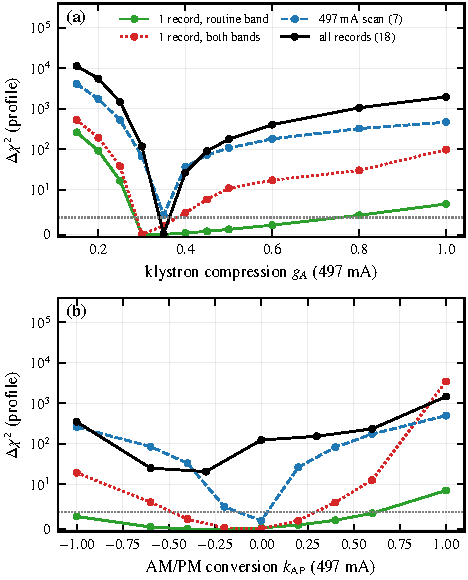
\includegraphics[width=\linewidth]{figures/identifiability}
\caption{Profile likelihood of the klystron's (a) amplitude compression $\gA$ and (b) AM/PM conversion $\kAP$ at the \SI{497}{mA} operating point, with both free at every operating point, for nested data sets: the loop band of one record (\SIrange{\fSplit}{\fHi}{kHz}), the same record over the full band, the gain and phase scan at \SI{497}{mA}, and all records. Every other parameter is re-optimized at each point; the dotted line marks the 95\% level ($\Delta\chi^2=3.84$). The vertical axis is linear below 10.}\label{fig:ident}
\end{figure}

\subsection{What the trip records add}\label{sec:trips}

The trip records measure the klystron without any loop model (App.~\ref{app:trips}). In the normal operation before each trip, the relative fluctuations of the klystron output amplitude follow those of the drive amplitude with a ratio of $\tripGA\pm\tripGAErr$ between 50 and \SI{200}{kHz} over the \tripUsed{} records (Fig.~\ref{fig:trips}a): $\tripGAFull\pm\tripGAFullErr$ at full output and $\tripGARed\pm\tripGARedErr$ at the no-beam output. The coherence is \tripCohLo--\tripCohHi, and the $H_2$ estimate, biased the other way by noise, gives \tripGAHtwo, so the ratio is the klystron's small-signal compression $\gA$. Below \SI{10}{kHz} it is \tripGALow, and above \SI{200}{kHz} it falls to $\tripGAHigh\pm\tripGAHighErr$, where the two measurement chains need not be flat. The probe's response to drive amplitude, relative to its response to drive phase, gives the AM/PM conversion: for a memoryless klystron and any plant that treats both quadratures alike the ratio is $\kAP-j\gA$, and the records give $\kAP=\tripKAP\pm\tripKAPErr$ (Fig.~\ref{fig:trips}b). The loop's own correlation pulls this ratio towards a linear klystron---the same regression returns $\gA=\tripGARatio$ instead of \tripGA---so $|\kAP|$ is if anything underestimated, by about a fifth. The values that the closed-loop records give with $\kAP$ free at every operating point, from \kapFreeLo{} to \kapFreeHi, lie far outside this range.

We therefore fix the AM/PM conversion at the trip-record value. This raises $\chi^2$ by \chiCostKap, \SI{\chiCostKapPct}{\percent} of its value, moves the compression at full current by at most \gaShiftHigh, and leaves the nuisance parameters regular: the noise angle, which depends only on the klystron's insertion phase, varies by \ang{\alphaSpread} between operating points instead of \ang{\alphaSpreadFree}.

\begin{figure*}[tb]
\centering
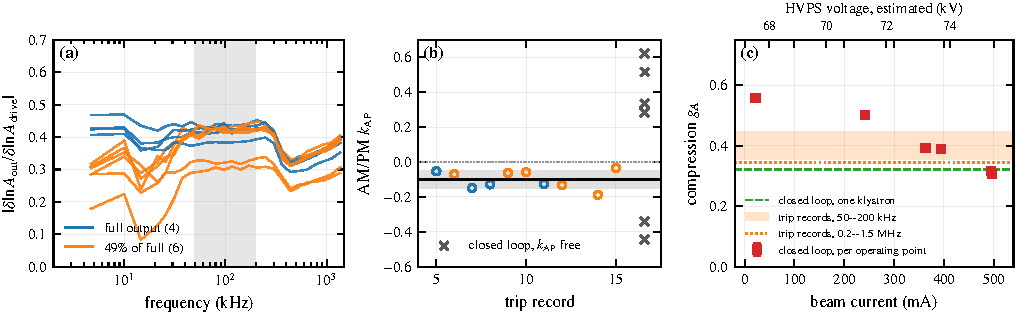
\includegraphics[width=\textwidth]{figures/trip_klystron}
\caption{The klystron in the trip records (present tube, 2021). (a) Ratio of the relative fluctuations of output and drive amplitude against frequency, for the records at full output (blue) and at the no-beam output (orange); shaded: \SIrange{50}{200}{kHz}. (b) AM/PM conversion from the probe's response to drive amplitude and phase, per record (band: mean $\pm$ standard deviation); crosses: the values of the closed-loop fit with $\kAP$ free at every operating point. (c) Compression identified from the closed-loop records at each operating point (squares) and as one value for all currents (dashed), against the trip records at \SIrange{50}{200}{kHz} (band) and above \SI{200}{kHz} (dotted); top axis: HVPS voltage estimated from the power balance at the fixed drive.}\label{fig:trips}
\end{figure*}

% ======================================================================================================
\section{Competing explanations}\label{sec:explain}
% ======================================================================================================

\subsection{The anomaly}

Fitted record by record with a complex-linear loop, the loop band of every record is described to within a few percent ($\chi^2/\nu=\chiLoopLinEff$), but the parameters drift with the operating point (Fig.~\ref{fig:effective}). At the operating gain setting, the effective loop gain falls from \effGLow{} at \SI{22}{mA} to \effGHigh{} at \SI{500}{mA}; the effective delay rises from \SI{\effTauLow}{ns} to \SIrange{\effTauHighLo}{\effTauHighHi}{ns}; the effective $\QL$ falls from about \effQLow{} to \effQHighLo--\effQHighHi. None of these is plausible for the hardware: the gain is held by gain tracking, the delay is cable and klystron transit time and was measured as \SI{\tauMeas}{ns}, and $\QL$ is fixed by the couplers and agrees at low current with the value from the reflected power. At \SI{497}{mA} the effective gain also scales more steeply than the gain setting, and at \SI{22}{mA} it changes with the phase setting---from \effGPhaseA{} to \effGPhaseB{} as the phase setting is lowered by \ang{\phaseScanLow}---which no rotation can do. The same records show the coupled beam mode as a resonance near $\pm f_s$ whose frequency falls from \modeFreeFHi{} to about \SI{\modeFreeFLo}{kHz} with current, and whose damping rate rises from about \SI{\dampHighGainFree}{} to \SI{\dampLowGainFree}{s^{-1}} as the gain is lowered by \SI{1.5}{dB} at \SI{497}{mA} (Fig.~\ref{fig:data}).

\begin{figure*}[tb]
\centering
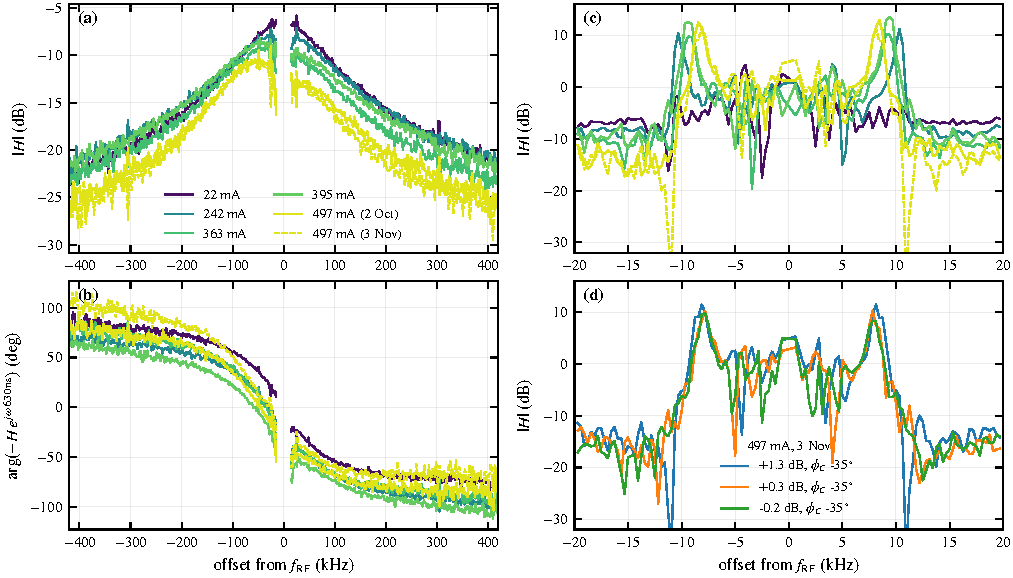
\includegraphics[width=\textwidth]{figures/data_overview}
\caption{Measured closed-loop responses, independent LPM estimates every \SI{\lpmWidth}{Hz} combined into data points as in the fits, through the carrier. (a) Magnitude and (b) phase over the full band (logarithmic offset axis, linear within \SI{0.5}{kHz}), the phase with \SI{630}{ns} of delay removed; colour: beam current; (I), (II): sessions. (c) The near band for the same records: the coupled mode appears as a resonance near $\pm f_s$ that moves down with current. (d) The near band at \SI{497}{mA} (session II) for three loop-gain settings, relative to the operating setting. Dotted: noise level, the standard deviation of the estimates, at 22 and \SI{497}{mA} (II) in (a) and (c) and for one record in (d); where it approaches $|H|$, near the carrier, the estimates scatter accordingly.}\label{fig:data}
\end{figure*}

\begin{figure*}[tb]
\centering
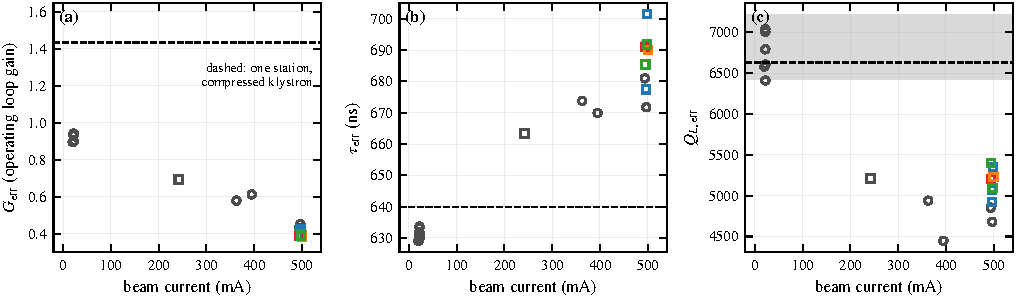
\includegraphics[width=\textwidth]{figures/effective_parameters}
\caption{Effective parameters of record-by-record complex-linear fits: (a) loop gain at the operating gain setting, (b) loop delay, (c) loaded $Q$. Circles: session I; squares: session II, coloured at \SI{497}{mA} by the loop-gain setting as in Fig.~\ref{fig:mode}(b). Dashed: the station constants of the selected model (Sec.~\ref{sec:selected}); grey band in (c): $\QL$ of the four cavities from their reflected power.}\label{fig:effective}
\end{figure*}

\subsection{Explanations and their test}

Table~\ref{tab:models} compares the candidate explanations, each fitted to all eighteen records over the full band (\nPoints{} real data points).
\begin{itemize}
\item \emph{One station, linear klystron.} Shared hardware, detuning from the data, beam dynamics included. It fails by more than an order of magnitude in both bands: the change of the response with current is not a beam-dynamics effect at fixed hardware.
\item \emph{Unequal cavity detunings.} A spread of the four detunings broadens the vector-sum response and could mimic a lower $\QL$. Fitted freely it reaches spreads of tens of kilohertz, which the measured reflected power of every cavity (1--3\%) excludes, and it still fails.
\item \emph{Effective parameters per record.} Per-record $G$, $\tau$ and $\QL$ describe the loop band as well as any model here ($\chi^2/\nu=\chiWideEff$) but not the near band (\chiBeamEff): at the coupled mode, between 5 and \SI{15}{kHz}, they leave \chiEffMode{} times the noise variance, against \chiSelMode{} for the selected model, because the damping of the coupled mode they imply is too small. They also lack a physical reading and do not transfer between conditions (Sec.~\ref{sec:valid}).
\item \emph{Compressed klystron.} Shared hardware, the klystron's compression and the noise angle per operating point, its AM/PM conversion from the trip records. With the momentum compaction identified (Sec.~\ref{sec:fs}) it describes the near band at the noise level ($\chi^2/\nu=\chiBeamSel$) and the loop band to within a few percent of $|H|$ (\chiWideSel) with \nparSel{} parameters; with the design value it fails in the near band and pulls the station constants away from their measured values. Variants test the klystron itself. Its compression and AM/PM taken from the trip records, with no klystron parameter fitted, already describe the records far better than any linear model ($\chi^2/\nu=\chiTrip$). One compression for all currents is worse ($\Delta\mathrm{AIC}=\daicOne$), and freeing the AM/PM conversion at every operating point lowers $\chi^2$ only by the amount discussed in Sec.~\ref{sec:trips}, with values that the trip records exclude. Without the beam's dipole motion the fit fails by far ($+\daicNobeam$).
\end{itemize}

\begin{table*}[tb]
\caption{Candidate explanations fitted to all records over the full band. The compressed-klystron models use the AM/PM conversion of the trip records unless stated. $n_p$: free parameters; $\chi^2/\nu$ overall and in the loop band (\SIrange{\fSplit}{\fHi}{kHz}) and the near band ($|f|<\SI{\fSplit}{kHz}$); $\Delta$AIC and $\Delta$BIC relative to the selected model~\cite{Akaike1974,Schwarz1978}.}\label{tab:models}
\begin{ruledtabular}
\begin{tabular}{lrrrrrr}
Model & $n_p$ & $\chi^2/\nu$ & loop band & near band & $\Delta$AIC & $\Delta$BIC \\
\hline
One station, linear klystron & \nparShared & \chiShared & \chiWideShared & \chiBeamShared & \daicShared & \dbicShared \\
\quad + unequal cavity detunings & \nparSpread & \chiSpread & \chiWideSpread & \chiBeamSpread & \daicSpread & \dbicSpread \\
Effective $G$, $\tau$, $\QL$ per record & \nparEff & \chiEff & \chiWideEff & \chiBeamEff & \daicEff & \dbicEff \\
Klystron of the trip records, none fitted & \nparTrip & \chiTrip & \chiWideTrip & \chiBeamTrip & \daicTrip & \dbicTrip \\
Compressed klystron, one for all currents & \nparOne & \chiOne & \chiWideOne & \chiBeamOne & \daicOne & \dbicOne \\
Per operating point, design $\alpha_c$ & \nparSelNom & \chiSelNom & \chiWideSelNom & \chiBeamSelNom & \daicSelNom & \dbicSelNom \\
Per operating point, no beam motion & \nparNobeam & \chiNobeam & \chiWideNobeam & \chiBeamNobeam & \daicNobeam & \dbicNobeam \\
Per operating point, AM/PM free & \nparFree & \chiFree & \chiWideFree & \chiBeamFree & \daicFree & \dbicFree \\
\textbf{Selected: compression per operating point} & \nparSel & \chiSel & \chiWideSel & \chiBeamSel & 0 & 0 \\
\end{tabular}
\end{ruledtabular}
\end{table*}

\begin{figure*}[tb]
\centering
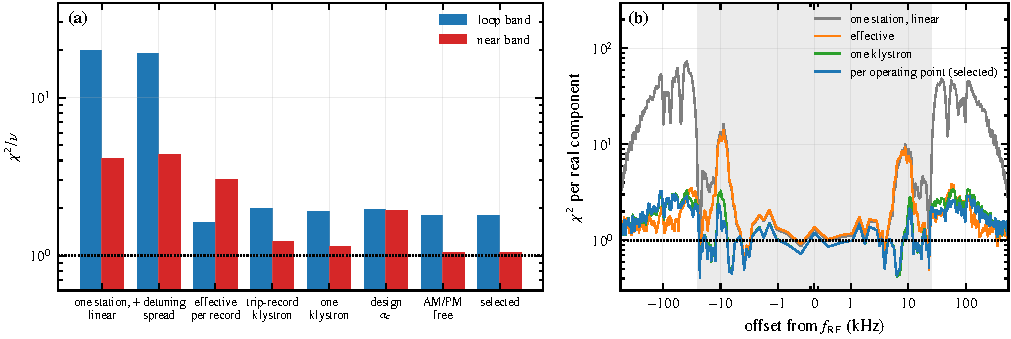
\includegraphics[width=\textwidth]{figures/model_comparison}
\caption{(a) $\chi^2/\nu$ of the candidate explanations of Table~\ref{tab:models} in the loop band and the near band (all records); the last three have the compression per operating point. (b) Squared normalized residuals per real component over the full band (shaded: near band), averaged over all records and over five adjacent data points; 1 is the noise level. The dips near $\pm\SI{22}{kHz}$ lie at interference lines, which raise the averaged noise level there.}\label{fig:models}
\end{figure*}

Figure~\ref{fig:models}(b) shows where the models fail. The linear station misses everywhere. In the near band the selected model is close to the noise level for every record ($\chi^2/\nu$ of \chiRecNearLo--\chiRecNearHi), the coupled mode included. In the loop band every model with a compressed klystron, and the effective model with three free parameters per record, leaves the same residual structure, a few percent of $|H|$ with opposite signs on the two sides of the carrier; it is largest between 25 and \SI{150}{kHz} ($\chi^2/\nu=\chiSelLoopLow$ for the selected model) and smaller above (\chiSelLoopHigh). It is worst in the two extreme settings of the low-current phase scan ($\chi^2/\nu$ of \chiRecLowLo{} and \chiRecLowHi{} over the full band, against at most \chiRecOthersHi{} and a median of \chiRecOthersMedian{} for the other records). Two physical causes were tested and rejected. A finite bandwidth of the klystron's amplitude path alone, between \fAlo{} and \SI{\fAhi}{MHz} with the phase path unchanged, worsens the fit by at least $\Delta\chi^2=\dchiFAmin$, so the fall of the trip-record compression above \SI{200}{kHz} (Sec.~\ref{sec:trips}) more likely belongs to the measurement chains than to the tube; and unequal loaded $Q$ of the four cavities, taken from their reflection (spread \qSpread\%), changes $\chi^2$ by \dchiQrel. The structure is common to all the explanations compared here and does not decide between them; it sets the accuracy of the model in the loop band.

\subsection{The selected model}\label{sec:selected}

The station constants are $G_0=\Gzero\pm\GzeroErr$, $\tau=\tauFit\pm\tauFitErr$~ns and $\QL=\QLFit\pm\QLFitErr$ (statistical errors). The delay is \SI{\tauDiff}{ns} longer than the \SI{\tauMeas}{ns} measured on the station~\cite{Sebek2026}, a difference that the excitation and recording paths outside the loop can account for: their linear phase is absorbed in $\tau$ (Sec.~\ref{sec:model}). $\QL$ lies within the range of the four cavities' loaded $Q$ from their reflection without beam (\QLreflLo--\QLreflHi, \QLrefl{} for their vector sum; Sec.~\ref{sec:system}). The measurement chain contributes an odd magnitude slope of \chainOdd~dB and an even phase of \ang{\chainEvenPh} at $\pm\SI{400}{kHz}$, common to all records. Table~\ref{tab:groups} lists the operating-point parameters. The detunings follow the beam-loading compensation, $\Delta f\approx-\SI{36}{kHz}\times\Ib/\SI{500}{mA}$, to within about \SI{3}{kHz}, as the tuners' load-angle offset allows. The loop phase at \SI{22}{mA} follows the phase setting with a slope of \thetaSlopeLow{} degrees per degree.

The klystron's compression grows with the beam current, from $\gA=\gaSelLow$ at \SI{22}{mA} through \gaSelMid{} at 242, 363 and \SI{395}{mA} to \gaSelHighLo--\gaSelHighHi{} at \SI{494}{}--\SI{497}{mA}, and the two high-current operating points, measured a month apart, agree within their errors. This is the trend that the station's operation implies: the drive is the same at every current, but with beam the tube runs at a higher voltage and much closer to saturation (efficiency \SI{\klyEffHigh}{\percent} against \SI{\klyEffLow}{\percent} without beam, Sec.~\ref{sec:system}). The HVPS voltage was not recorded with the closed-loop records. Estimated from the power balance at the fixed drive---cavity losses, beam power and the reflection at the cavities' coupling $\beta\approx\betaMean$, scaled by \pfwdScale{} to the snapshots and interpolated between their voltages---it rises from about \SI{\vkLow}{kV} at \SI{22}{mA} through \vkMid{}~kV to \SI{\vkHigh}{kV} at \SI{494}{}--\SI{497}{mA} (Table~\ref{tab:groups}), and the compression falls monotonically with it. The phase path of the loop therefore has the gain $G_0=\Gzero$ at the operating setting, while a perturbation of the drive amplitude meets a loop gain of only $\gA G_0\approx\ampLoopHigh$ at \SI{500}{mA}. The effective loop gain of about \effGLow{} that a complex-linear fit returns at low current (Fig.~\ref{fig:effective}a) is neither of the two but their projection on the direction of the injected noise [Eq.~\eqref{eq:recorded}].

\begin{table*}[tb]
\caption{Records and operating-point parameters of the selected model. Sessions I and II were a month apart; $n$: number of records; $\Delta G$, $\Delta\phi$: loop-gain and loop-phase settings relative to the operating settings; $V_k$: HVPS voltage, not recorded, estimated from the power balance at the fixed drive (Sec.~\ref{sec:selected}); $\gA$: klystron compression (statistical errors); $\alpha$: noise angle in the cavity frame; $\Delta f$: detuning of each group of records taken minutes apart. The AM/PM conversion is fixed at $\kAP=\kapTrip$ (trip records, Sec.~\ref{sec:trips}).}\label{tab:groups}
\begin{ruledtabular}
\begin{tabular}{lcccccccc}
Session & $\Ib$ (mA) & $n$ & $\Delta G$ (dB) & $\Delta\phi$ ($^\circ$) & $V_k$ (kV) & $\gA$ & $\alpha$ ($^\circ$) & $\Delta f$ (kHz) \\
\hline
I & 22 & 6 & $-0.4$ & $-3$ to $+6$ & 67 & $0.56\pm0.01$ & $-12$ & $-1.9$, $-1.8$, $+1.0$ \\
I & 363 & 1 & $-0.4$ & $-3$ & 73 & $0.40\pm0.01$ & $-16$ & $-24.2$ \\
I & 395 & 1 & $-0.4$ & $+0$ & 74 & $0.39\pm0.01$ & $-23$ & $-27.9$ \\
I & 496 & 2 & $-0.4$ & $-3$ to $+0$ & 75 & $0.32\pm0.01$ & $-11$ & $-33.1$ \\
II & 242 & 1 & $+0.0$ & $+0$ & 71 & $0.49\pm0.01$ & $-14$ & $-18.2$ \\
II & 497 & 7 & $-1.5$ to $+0.0$ & $-15$ to $-10$ & 75 & $0.31\pm0.01$ & $-4$ & $-33.2$

\end{tabular}
\end{ruledtabular}
\end{table*}

\begin{figure*}[tb]
\centering
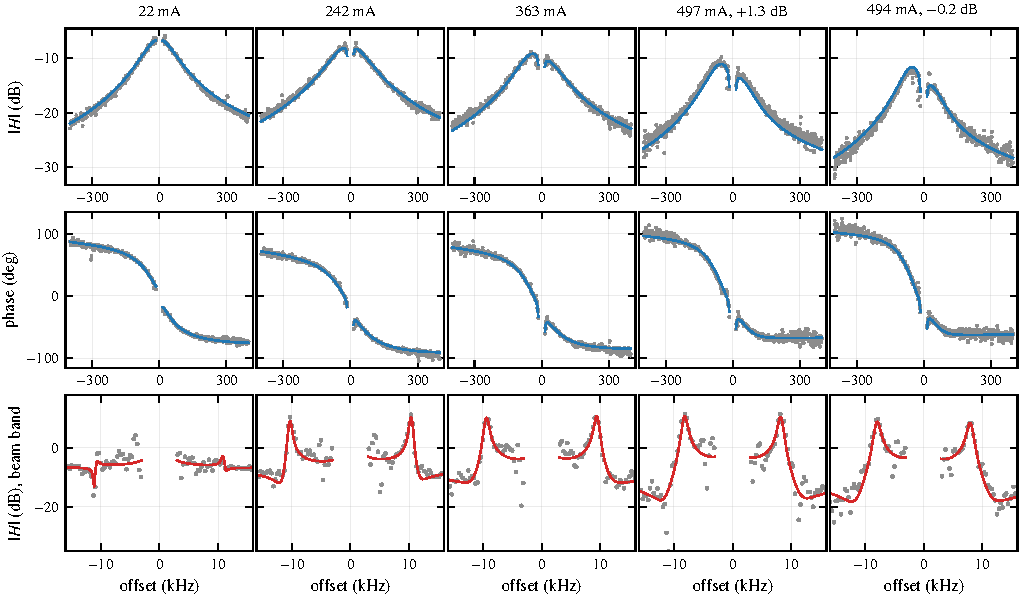
\includegraphics[width=\textwidth]{figures/fits}
\caption{Recorded responses (grey) and the selected model (lines) for five operating points, labelled by beam current and, at \SI{497}{mA} (session II), loop-gain setting: magnitude and phase over the full band (top, middle; phase with \SI{630}{ns} removed) and magnitude in the near band (bottom; shaded: the model $\pm$ the standard deviation of the estimates, the scatter expected of the data). The model is averaged over the \SI{\lpmWidth}{Hz} of each estimate. One set of station constants describes all records.}\label{fig:fits}
\end{figure*}

% ======================================================================================================
\section{Validation}\label{sec:valid}
% ======================================================================================================

\subsection{Out-of-band prediction of the coupled mode}\label{sec:fs}

The first test asks whether the loop identified in the loop band alone predicts the coupled mode, which lives in a band that was not used. For each of the \nModeRecs{} records with more than \SI{200}{mA}, the coupled mode is measured without a model by fitting a pole pair and a smooth background to both sides of the near band between 3 and \SI{16}{kHz} (App.~\ref{app:estimator}); frequencies are determined to about \SI{\modeFreeDf}{Hz} and damping rates to about \SI{\modeFreeDs}{s^{-1}}. The models are then evaluated with no adjustment.

Both loop-band models fail, in opposite ways (Fig.~\ref{fig:mode}a). The effective linear model places the mode at about the right frequency (mean error \oobEffDf~Hz) but with too little damping (mean error \oobEffDs~s$^{-1}$, rms \oobEffDsRms~s$^{-1}$): its effective parameters describe the projection that the routine measures, not the impedance that the beam sees. The compressed-klystron model gets the damping roughly right (mean error \oobWlDs~s$^{-1}$)---the klystron's compression supplies the damping that a linear model lacks---but places the mode \oobWlDfAbs~Hz too low. The prediction thus isolates one discrepancy, the coherent frequency, in a model whose loop is otherwise right.

The coherent frequency at fixed loop depends on the beam through $\omega_s^2$ and $\kappa_1I_{b1}$, both proportional to $\alpha_c$. The mode at \SI{242}{mA}, at \modeFreeFHi~kHz, already lies above the nominal incoherent frequency $f_s=\fsNom$~kHz, whereas in every model considered here the reactive loading of cavities tuned below $\fRF$ pulls the coherent mode below $f_s$. Identifying $\alpha_c$ jointly with the loop, from the full band, gives $\alpha_c=\alphacFit\times10^{-3}$, with a statistical error of \alphacFitErr$\times10^{-3}$ and a range of \alphacLo--\alphacHi$\times10^{-3}$ over the compressed-klystron models of Table~\ref{tab:models} that leave it free, i.e., an incoherent synchrotron frequency of \fsFit~kHz at \SI{2.85}{MV} (\fsLo--\fsHi~kHz), \fsRatio\% above the nominal value. With the design value the fit worsens in both bands ($\chi^2/\nu=\chiWideSelNom$ and \chiBeamSelNom{} against \chiWideSel{} and \chiBeamSel), and the station constants move away from their measured values ($\QL=\QLSelNom$, $\tau=\SI{\tauSelNom}{ns}$). Two alternatives were tested. Freeing the beam-coupling strength separately from $\omega_s$ returns a coupling factor $\kscale\pm\kscaleErr$ with $\alpha_c=\alphacKs\times10^{-3}$: both scale as $\alpha_c$ does, which a calibration error of the gap voltage (acting on $\omega_s$ alone) would not produce. And the effective linear model does not improve with $\alpha_c$ free: its deficit is the damping. With $\alpha_c$ identified the coupled mode agrees with the model-free poles to \jointDfRms~Hz in frequency and \jointDsRms~s$^{-1}$ in damping (rms over \nModeRecs{} records), across currents from 242 to \SI{500}{mA} and loop-gain settings down to \SI{\gainDropMax}{dB} below the operating setting (Fig.~\ref{fig:mode}); with one compression for all currents the damping comes out \jointOneDsAbs~s$^{-1}$ too high on average. The identified value lies \alphacAboveLo--\alphacAboveHi\% above the published lattice values, $1.18\times10^{-3}$ for the operating lattice~\cite{Huang2007} and $1.13\times10^{-3}$ in the design report~\cite{Hettel2002}; it is either a property of the present lattice or a proxy for an unmodelled element that acts on the coupled mode like a stronger synchrotron focusing. A direct measurement of the incoherent synchrotron frequency at a few milliamperes, where the coherent shift vanishes, decides between the two: the model predicts \fsFit~kHz.

\begin{figure*}[tb]
\centering
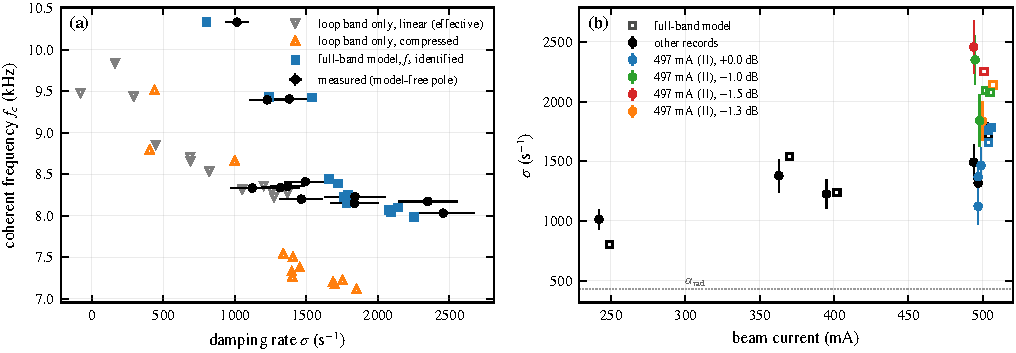
\includegraphics[width=\textwidth]{figures/coupled_mode}
\caption{The coupled beam--cavity--klystron--loop mode. (a) Frequency and damping rate measured without a model (black, $1\sigma$ errors), predicted from the loop band alone by the effective linear model (grey) and by the compressed-klystron model with nominal ring parameters (orange), and given by the full-band model with the synchrotron frequency identified (blue). (b) Damping rate against beam current, measured (filled) and from the full-band model (open squares); at \SI{497}{mA} (session II) the colours mark the loop-gain setting relative to the operating setting. Dotted: radiation damping.}\label{fig:mode}
\end{figure*}

\subsection{Prediction across operating conditions}

The second test asks whether the identified model predicts records taken under conditions it was not trained on. Each model is refitted without the held-out records; for these only nuisance parameters are refitted: the loop phase, plus the detuning (and the noise angle, for the klystron models) when the beam current is new. The effective model needs its per-record parameters at the new condition: they are taken from the same operating point and scaled with the gain setting (gain transfer), averaged over the neighbouring phase settings (phase transfer), or interpolated in beam current (current transfer); the selected model interpolates $\gA$ in beam current, and the single klystron needs nothing. Figure~\ref{fig:crossval} shows the held-out $\chi^2/\nu$.

For a new beam current the selected model predicts the record almost as well as it fits it in sample: \cvIaSel, \cvIbSel{} and \cvIcSel{} at 242, 363 and \SI{395}{mA}, against \cvIaIn, \cvIbIn{} and \cvIcIn{} in sample; the single klystron gives \cvIaOne, \cvIbOne{} and \cvIcOne, and interpolated effective parameters give \cvIaEff, \cvIbEff{} and \cvIcEff. For new gain settings at \SI{497}{mA} the selected model gives \cvGainSel{} on average (in sample \cvGainIn) and the scaled effective model \cvGainEff, the difference lying in the near band (\cvGainNearSel{} against \cvGainNearEff{} per record). For new phase settings at \SI{22}{mA} both give about 3 (\cvPhaseSel{} and \cvPhaseEff), close to the selected model's in-sample value of these two records (\cvPhaseIn). Freeing the AM/PM conversion at every operating point changes no prediction materially (\cvIaFree, \cvIbFree, \cvIcFree; \cvGainFree; \cvPhaseFree). The one-station linear model fails every test.

\begin{figure}[tb]
\centering
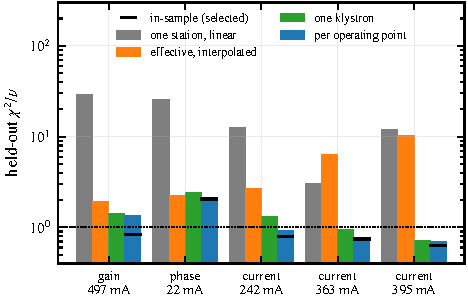
\includegraphics[width=\linewidth]{figures/crossval}
\caption{Held-out $\chi^2/\nu$ (full band) of records predicted from models trained without them: gain transfer at \SI{497}{mA} (four records), phase transfer at \SI{22}{mA} (two), and three beam currents. Bars: one-station linear model, effective model with transferred parameters, one compressed klystron for all currents, compression per operating point (selected). Black ticks: in-sample values of the selected model.}\label{fig:crossval}
\end{figure}

\subsection{Comparison with the trip records}\label{sec:tripcomp}

At full current the identified compression, \gaSelHighLo--\gaSelHighHi{} at \SI{494}{}--\SI{497}{mA} (\gaFreeHigh{} with the AM/PM conversion free), lies below the trip-record value at full output, $\tripGAFull\pm\tripGAFullErr$ at \SIrange{50}{200}{kHz}, and close to the trip-record value above \SI{200}{kHz}, $\tripGAHigh\pm\tripGAHighErr$ (Fig.~\ref{fig:trips}c). Both describe a strongly compressed klystron: a change of the drive amplitude reaches the output with a third to two fifths of its relative size. At low output the two disagree. The trip records give $\tripGARed\pm\tripGARedErr$ at the no-beam output, where the closed-loop records give \gaSelLow{} at \SI{22}{mA}; in the trip records the compression hardly depends on the output, in the closed-loop records it does. A single compression for all currents, \gaOneKly, costs $\Delta\chi^2=\dchiOne$: \dchiOneLow{} from the \SI{22}{mA} records, \dchiOneMid{} from the single records at 242--\SI{395}{mA}, and \dchiOneHigh{} from the eleven records at 494--\SI{497}{mA}. The current dependence thus rests on the low-current phase scan, which no model reproduces at the noise level in its extreme settings, and on the records at intermediate current, among them the near band at 242 and \SI{363}{mA}, where a single compression overestimates the damping. It is the trend expected from the klystron's efficiency at the two voltages (Sec.~\ref{sec:selected}). The trip records are five years older, and their beam currents, cathode voltages and loop settings were not recorded; a transfer-curve measurement at the present drive and at the cathode voltages of low and high current would settle the point. Taken as they are, with no klystron parameter fitted, the trip-record values describe all eighteen records better than any linear model ($\chi^2/\nu=\chiTrip$, Table~\ref{tab:models}).

\subsection{Physical consistency}

The station constants agree with independent knowledge: $\tau$ with the delay measured on the station, to within the delay outside the loop, $\QL$ with the reflected power, the detunings with the beam-loading compensation, the gain constant across operating points with the gain tracking, the loop-phase slope at low current with the earlier calibration, and the growth of the compression with the klystron's efficiency. None of these was imposed.

% ======================================================================================================
\section{Discussion}\label{sec:disc}
% ======================================================================================================

\paragraph{What changes with the beam.} The dominant change of the loop dynamics between \SI{20}{} and \SI{500}{mA} is the compression of the klystron, which runs closer to saturation as the HVPS raises its voltage to supply the beam's power at a fixed drive; the detuning and the beam's dipole motion are the other two current-dependent elements, and both follow from physics once the loop is known. A complex-linear model can follow the change only with effective parameters that mean nothing physical, and such a model does not predict the coupled mode or new operating points. The compression divides the loop into two: a phase loop of gain $G_0\approx\Gzero$ and an amplitude loop of about one third of that at \SI{500}{mA} ($\gA G_0\approx\ampLoopHigh$). The weaker amplitude loop leaves more of the cavity's natural impedance to the beam, and that supplies the Robinson damping that a linear model cannot: identified on the loop band alone, the linear model with effective parameters underestimates the damping of the coupled mode by about \SI{\oobEffDsAbs}{s^{-1}} on average (Sec.~\ref{sec:fs}). Lowering the gain by \SI{1.5}{dB} at \SI{497}{mA} raises the measured damping rate from about \SI{\dampHighGainFree}{} to \SI{\dampLowGainFree}{s^{-1}}; the model reproduces the direction and \dampChangePct\% of the size of this change (\SI{\dampHighGainModel}{} to \SI{\dampLowGainModel}{s^{-1}}), but at the highest gain it overestimates the damping by about \SI{\dampHighGainOver}{s^{-1}}, \dampOverRatio{} times the measurement error.

\paragraph{The synchrotron frequency.} The near band identifies a combination of beam parameters that the loop band cannot, and the result disagrees with the design value by \fsRatio\% in $f_s$. Because the incoherent synchrotron frequency is easy to measure at low current, this is a falsifiable prediction; if it is confirmed, the momentum compaction of the present lattice should be revised in every longitudinal model of the ring; if not, the coupled-mode band contains dynamics that the model lacks, most likely in the integral path or the klystron at a few kilohertz.

\paragraph{Limits.} The model assumes rigid bunches and a uniform fill, equal vector-sum weights and a memoryless klystron, and it treats the measurement chain as a smooth common factor. The loop phase of each record is a free parameter because the tracking correction was not recorded. The AM/PM conversion is taken from trip records five years older than the closed-loop data, because the closed-loop records determine it only together with the high-current loop phase; its value is small, and the compression at full current hardly depends on it. In the loop band the model leaves a residual of a few percent of $|H|$, common to all the explanations tested and largest in the low-current phase scan; neither a finite klystron bandwidth nor unequal cavity $Q$ explains it. Operating-point parameters for currents with a single record rest on that record, and the HVPS voltages of the operating points between \SI{0}{} and \SI{500}{mA} are estimated, not measured.

\paragraph{Measurements that would add most.} A two-dimensional excitation---independent noise sequences on I and Q, or a multisine whose lines sit on one side of the carrier---would measure $H_1$ and $H_2$ separately and determine the AM/PM conversion from the closed-loop records themselves. Longer records, or more excitation within a few kilohertz of the carrier, would raise the signal-to-noise ratio of the near band above the \snrNearLo--\SI{\snrNearHi}{dB} per estimate of these records (Sec.~\ref{sec:estimation}) and sharpen the coupled mode accordingly. The klystron's transfer curves (AM/AM and AM/PM) at the present drive and at the cathode voltages of low and high current would test the identified growth of the compression with current, which the older trip records do not show. Recording the HVPS voltage and the klystron's drive and output power with every closed-loop record would tie each record to its point on those curves, and recording the total loop phase would remove one nuisance parameter per record. The incoherent synchrotron frequency at low current settles the question of $\alpha_c$. With these, the same routine records would give a complete, predictive model of the station---and, for the replacement LLRF system, whose loop delay is longer, a quantitative basis for setting its gain and phase.

% ======================================================================================================
\section{Conclusions}\label{sec:concl}
% ======================================================================================================

Operational closed-loop measurements, taken with an existing diagnostic routine and a one-dimensional excitation, identify a compact physics-informed model of the coupled beam--cavity--klystron--feedback system of the SPEAR3 RF station. One set of station constants---loop gain, delay, loaded $Q$---describes eighteen records from 20 to \SI{500}{mA}, at several loop gains and phases, in two sessions a month apart, once the klystron is allowed to compress its amplitude response as it approaches saturation: at the noise level in the band of the coupled mode and to within a few percent of the response across the loop band. The constants agree with independent station data. Single records do not determine the klystron's asymmetry; records at several loop settings and the near band determine its compression, and trip records of the same tube supply its small AM/PM conversion, which the closed-loop records leave correlated with the loop phase. The compression grows with the beam current as the tube, held at a fixed drive, works closer to saturation; at full current it agrees with the trip records to within their spread across frequency bands, while the trip records show less dependence on the output power. Explanations by effective linear parameters, by unequal cavity detunings, or by beam dynamics at fixed hardware are rejected by the data. The identified model predicts records at beam currents it was not trained on almost at in-sample quality, where interpolated effective parameters fail. Its out-of-band prediction of the coupled beam mode isolated the one beam parameter that the loop band cannot determine; identified from the near band, it implies an incoherent synchrotron frequency \fsRatio\% above the design value, whatever the klystron model, a prediction that a simple low-current measurement can test. The physics supplied the structure; the data determined the klystron's compression, the station constants and the synchrotron focusing, and tested every explanation against measurements it was not built from.
